\chapter{Background}
\label{ch:Background}

\begin{citazione}
 L'informazione è il petrolio del 21° secolo e l'analisi è il motore a combustione. Peter Sondergaard~\cite{peter_sondergaard_cyte}
\end{citazione}

Sicuramente, tra i vari processi di trasformazione digitale, il principale è stato quello di dematerializzazione dei documenti cartacei, che prende il nome di \textbf{digitalizzazione} (o \textit{digitalization}). Più precisamente quando si parla di digitalizzazione si parla del processo di trasformazione di un'immagine, di un suono, di un documento in un formato digitale, interpretabile da un computer.~\cite{wikipedia_digitalization_definition}

A seguito di tale processo, le informazioni nel formato digitale (prendendo poi il nome di \textit{dato}), che in precedenza non era stato nemmeno immaginato, hanno acquisito sempre più importanza nel mondo fino a diventare uno, se non il, valore più importante.

\section{Incremento dei dati}
Fu compreso fin dal primo momento dell'ideazione di tale progetto di digitalizzazione, con lo scopo di riorganizzare la conoscenza in modo sempre più efficiente semplificando la selezione delle notizie in un mondo sommerso dalle informazioni, quanto questo fosse ambizioso, tuttavia, forse in parte venne sottostimato quale potesse essere la portata di tale rivoluzione. Tale idea ha portato non solo alla ridistribuzione e organizzazione delle informazioni pregresse, ma anche alla creazione di nuove informazioni dovute proprio a tale processo di modernizzazione. A queste, si sono poi aggiunte sempre più dati da dover salvare e gestire con l'incremento delle nuove tecnologie messe a disposizione dal progresso evolutivo che il mondo stava e sta tutt'ora affrontando. 

\subsection{Nuove dimensioni}

Proprio a causa dell'aumento di sempre nuovi dati e quindi del peso che questi occupino all'interno di uno spazio di memoria, è stato necessario ingrandire la scala delle unità di misura, creandone sempre più grandi tali da permettere di esprimere immediatamente la dimensione del volume di dati a cui si stesse facendo riferimento. Di seguito è riportata la tabella delle dimensioni attualmente definite.~\cite{datadrivendaily_dimension_table}

\begin{table}[hbt!]
    \centering
    \begin{tabular}{ccc}
        \hline
        Unità di misura & Abbreviazione & Dimensione\\
        \hline
        Bit & b & 1 o 0\\
        Byte & B & 8 b\\
        Kilobyte & KB & 1024 Byte o 210 bit\\
        Megabyte & MB & 1024 Kilobyte o 220 bit\\
        Gigabyte & GB & 1024 Megabyte o 230 bit\\
        Terabyte & TB & 1024 Gigabyte o 240 bit\\
        Petabyte & PB & 1024 Terabyte o 250 bit\\
        Exabyte & EB & 1024 Petabyte o 260 bit\\
        Zettabyte & ZB & 1024 Exabyte o 270 bit\\
        Yottabyte & YB & 1024 Zettabyte o 280 bit\\
    \end{tabular}
    \caption{Tabella delle unità di misura per l'espressione di dati}
    \label{tab:data_measures}
\end{table}

\subsection{La Digital DataSphere}

L'azienda IDC \footnote{La \textit{International Data Corporation} (\textit{IDC}) è un fornitore globale di informazioni di mercato, servizi di consulenza ed eventi per i mercati della tecnologia dell'informazione, delle telecomunicazioni e della tecnologia di consumo.} ha localizzato e definito i tre principali ambienti dove la digitalizzazione avviene di continuo e dove tali dati vengono salvati, ovvero:~\cite{idc_digital_datasphere}

\begin{enumerate}
    \item \textit{Core} (o “nucleo”): consiste nei datacenter tradizionali e cloud messi a disposizione dai provider;
    \item \textit{Edge} (o “bordo”): ovvero le infrastrutture delle imprese/aziende che non fanno parte dei datacenter principali; 
    \item \textit{Endpoint} (o “estremo”): con il termine "endpoint" si fa riferimento a tutti i dispositivi personali che sono agli estremi della rete, come PC, smartphone, dispositivi IoT, eccetera. 
\end{enumerate}

\begin{comment}
\begin{figure}[!h]
    \centering
    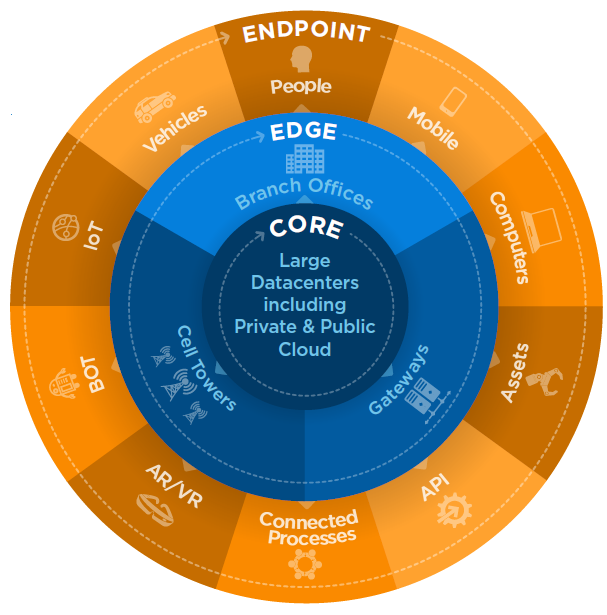
\includegraphics[width=0.5\linewidth]{figure/capitolo_2/Digital-Datasphere.png}
    \caption{Digital DataSphere}
    \label{fig:Digital-Datasphere}
\end{figure}
\end{comment}

La somma di tutti questi dati forma ciò che loro definiscono come \textbf{Global DataSphere}; più precisamente la Global DataSphere quantifica ed analizza l'ammontare dei dati creati, recuperati e duplicati in un dato anno nell'intero mondo.~\cite{datadrivendaily_dimension_table}

Secondo uno studio del 2018 svolto sull'incremento di tale Global DataSphere~\cite{idc_global_datasphere}, la IDC ha denotato un andamento al quanto impressionante di tipo esponenziale, ovvero secondo le stime entro il 2025 l'ammontare dei dati generati nell'intero mondo sarà pari a 175 ZB rispetto ai “soli” 80 del 2022. Leggendo il grafico riportato di seguito, è possibile notare che nel triennio 2023-2025 è stata stimato l'ammontare di 430 Zettabyte di dati, mentre andando dal 2022 a ritroso l'ammontare totale è minore di 400; in altre parole, i dati dell'ultimo triennio superano il totale dei dati creati fino al 2022 dall'inizio della storia della digitalizzazione. Per poter comprendere meglio e farsi un'ida di quanto questo valore sia elevato, riporto qui un esempio: se volessimo scaricare l'intero DataSphere del 2025, ovvero 175 ZB di dati, con una connessione di 100 Mb/s \footnote{Il valore preso in esempio è stato ricavato facendo riferimento alla media italiana di velocità di download, verificata nel 2022 ~\cite{github_speed_connection}, e poi approssimato per semplicità di calcolo} sarebbero necessari 554.552.923 anni (o più “semplicemente” 5.545.529 secoli) per completare l'operazione.

\begin{comment}
\begin{figure}[!h]
    \centering
    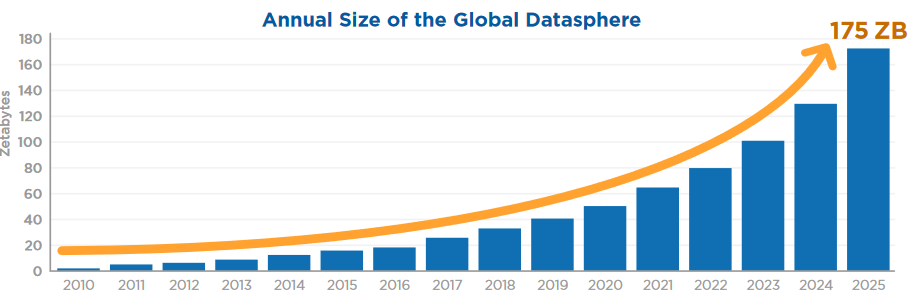
\includegraphics[width=1\linewidth]{figure/capitolo_2/Annual Size Global Datasphere.png}
    \caption{Dimensione annuale della Digital Datasphere globale}
    \label{fig:Annual Size Global Datasphere}
\end{figure}
\end{comment}

\subsection{Salvataggio e gestione dei dati}

Naturalmente, come è possibile dedurre autonomamente, questo incremento della generazione dei dati è dovuto a multipli fattori, su tutti sicuramente l'aumento di dispositivi a disposizione per la generazione di tali dati e l'espansione nel mondo dell'Internet e del Web con tutti i relativi servizi annessi. Attualmente siamo in un'era dove l'immensa quantità di dispositivi a nostra disposizione danno la possibilità alle persone di eseguire un'enorme quantità di azioni e interazioni, che non fanno altro che generare ulteriori dati e informazioni. L'incremento di tali dati ha generato in questo modo anche la necessità di salvarli e gestirli. Lo storage dei dati è la raccolta e la conservazione di informazioni digitali, tale processo svolge un ruolo sempre più centrale nella gestione dei dati e dei Big Data.~\cite{redhat_data_storage}

Più precisamente quando si parla di gestione dei dati si riferisce al processo di acquisizione, archiviazione e utilizzo dei dati che consente di sapere quali dati sono disponibili, dove si trovano, chi ne è il proprietario, chi può vederli e chi vi può accedere. La gestione dei dati consente alle organizzazioni di eseguire il deployment delle applicazioni e dei sistemi critici in modo sicuro e conveniente e di facilitare le decisioni strategiche.~\cite{redhat_data_management}

\section{Data-Driven Orientation}

Un aspetto molto importante ma che purtroppo viene molto sottovalutato all'interno delle aziende è la conoscenza reale del dato ancora prima della sua fruizione. Questo poiché non è possibile estrapolare informazioni da dati che si hanno a disposizione se non si ha una idea chiara su cosa essi possano effettivamente indicare e valorizzare. Proprio per sopperire a tale problematica, ormai l'approccio \textit{data-driven}, o \textit{data oriented}, è diventato sempre più comune nella maggior parte delle aziende.

\subsection{Il processo decisionale basato sui dati}

La strategia di effettuare delle decisioni basate sui dati è stata introdotta per puntualizzare la necessità di questo nuovo orientamento che considera la raccolta dei dati come un punto cardine delle strategie aziendali. L'adozione di un insieme integrato di tecnologie apposite per l'analisi dei dati può contribuire a facilitare la comunicazione in tempo reale, coinvolgere gli attori nella presa di decisioni e consentire la costante ridefinizione delle interazioni tra gli utenti e la tecnologia così da migliorare il benessere ed ottenere, con l'avanzare del tempo, innovazione e resilienza.~\cite{emerald_data_driven_orientation}

Più precisamente, il \textit{processo decisionale basato sui dati} (\textit{data-driven decision making, DDDM}) si definisce come l'utilizzo di elementi concreti, metriche e dati per orientare il processo decisionale aziendale in linea con obiettivi, scopi e iniziative. Cambiare il modo in cui la tua azienda prende decisioni non è semplice, ma incorporare dati e analisi nei cicli decisionali è il modo più efficace per generare il massimo dell'evoluzione dell'organizzazione. Proprio per questo motivo, per un'organizzazione è necessario rendere il processo decisionale data-driven una prassi.~\cite{tableau_data_driven_decision_making}

\subsection{Punti chiave delle aziende data-driven}
Le aziende data-driven basano la loro organizzazione su cinque punti chiave:~\cite{researchgate_data_driven_orientation}

\begin{enumerate}
    \item \textit{Digital transformation}. Per poter integrare i dati all'interno dei processi decisionali è necessario che questi siano naturalmente presenti e disponibili. Per permettere ciò è necessaria una chiara strategia di trasformazione digitale.
    \item \textit{Data science}. Con l'avvento dell'adozione di strumenti tecnologici, il modo in cui le organizzazioni producono, condividono e sfruttano i dati è cambiato. Per tale motivo la Data Science (è lo studio dei dati per estrarre informazioni significative per il business ) ha trovato nuovi modi per analizzare e ottenere valore dai dati.
    \item \textit{Data-Driven business model}. Al fine di generare ulteriore valore economico, le intuizioni aziendali acquisite devono essere sfruttate all'interno dei modelli di business. Una parte cruciale di questo processo è proprio la creazione di valore dalle informazioni digitalizzate, definendo come un DDBM si basi principalmente sul vedere i dati come una risorsa economicamente importante su cui investire.
    \item \textit{Data-Driven innovation}. Le aziende utilizzano i dati, da loro generati e raccolti, per trasformare le loro attività commerciali in innovazioni basate su questi. Attraverso tale innovazione, le organizzazioni sono abilitate ad utilizzare, e gestire coerentemente, le loro enormi quantità di dati (Big Data).
    \item \textit{Data Analytics}. Il valore dei dati ricercato deriva da un'attenta, corretta e congruente analisi dei dati a disposizione. Tale analisi permette alle compagnie di incrementare al meglio le proprie conoscenze aziendali.
\end{enumerate}

\begin{comment}
\begin{figure}[!h]
    \centering
    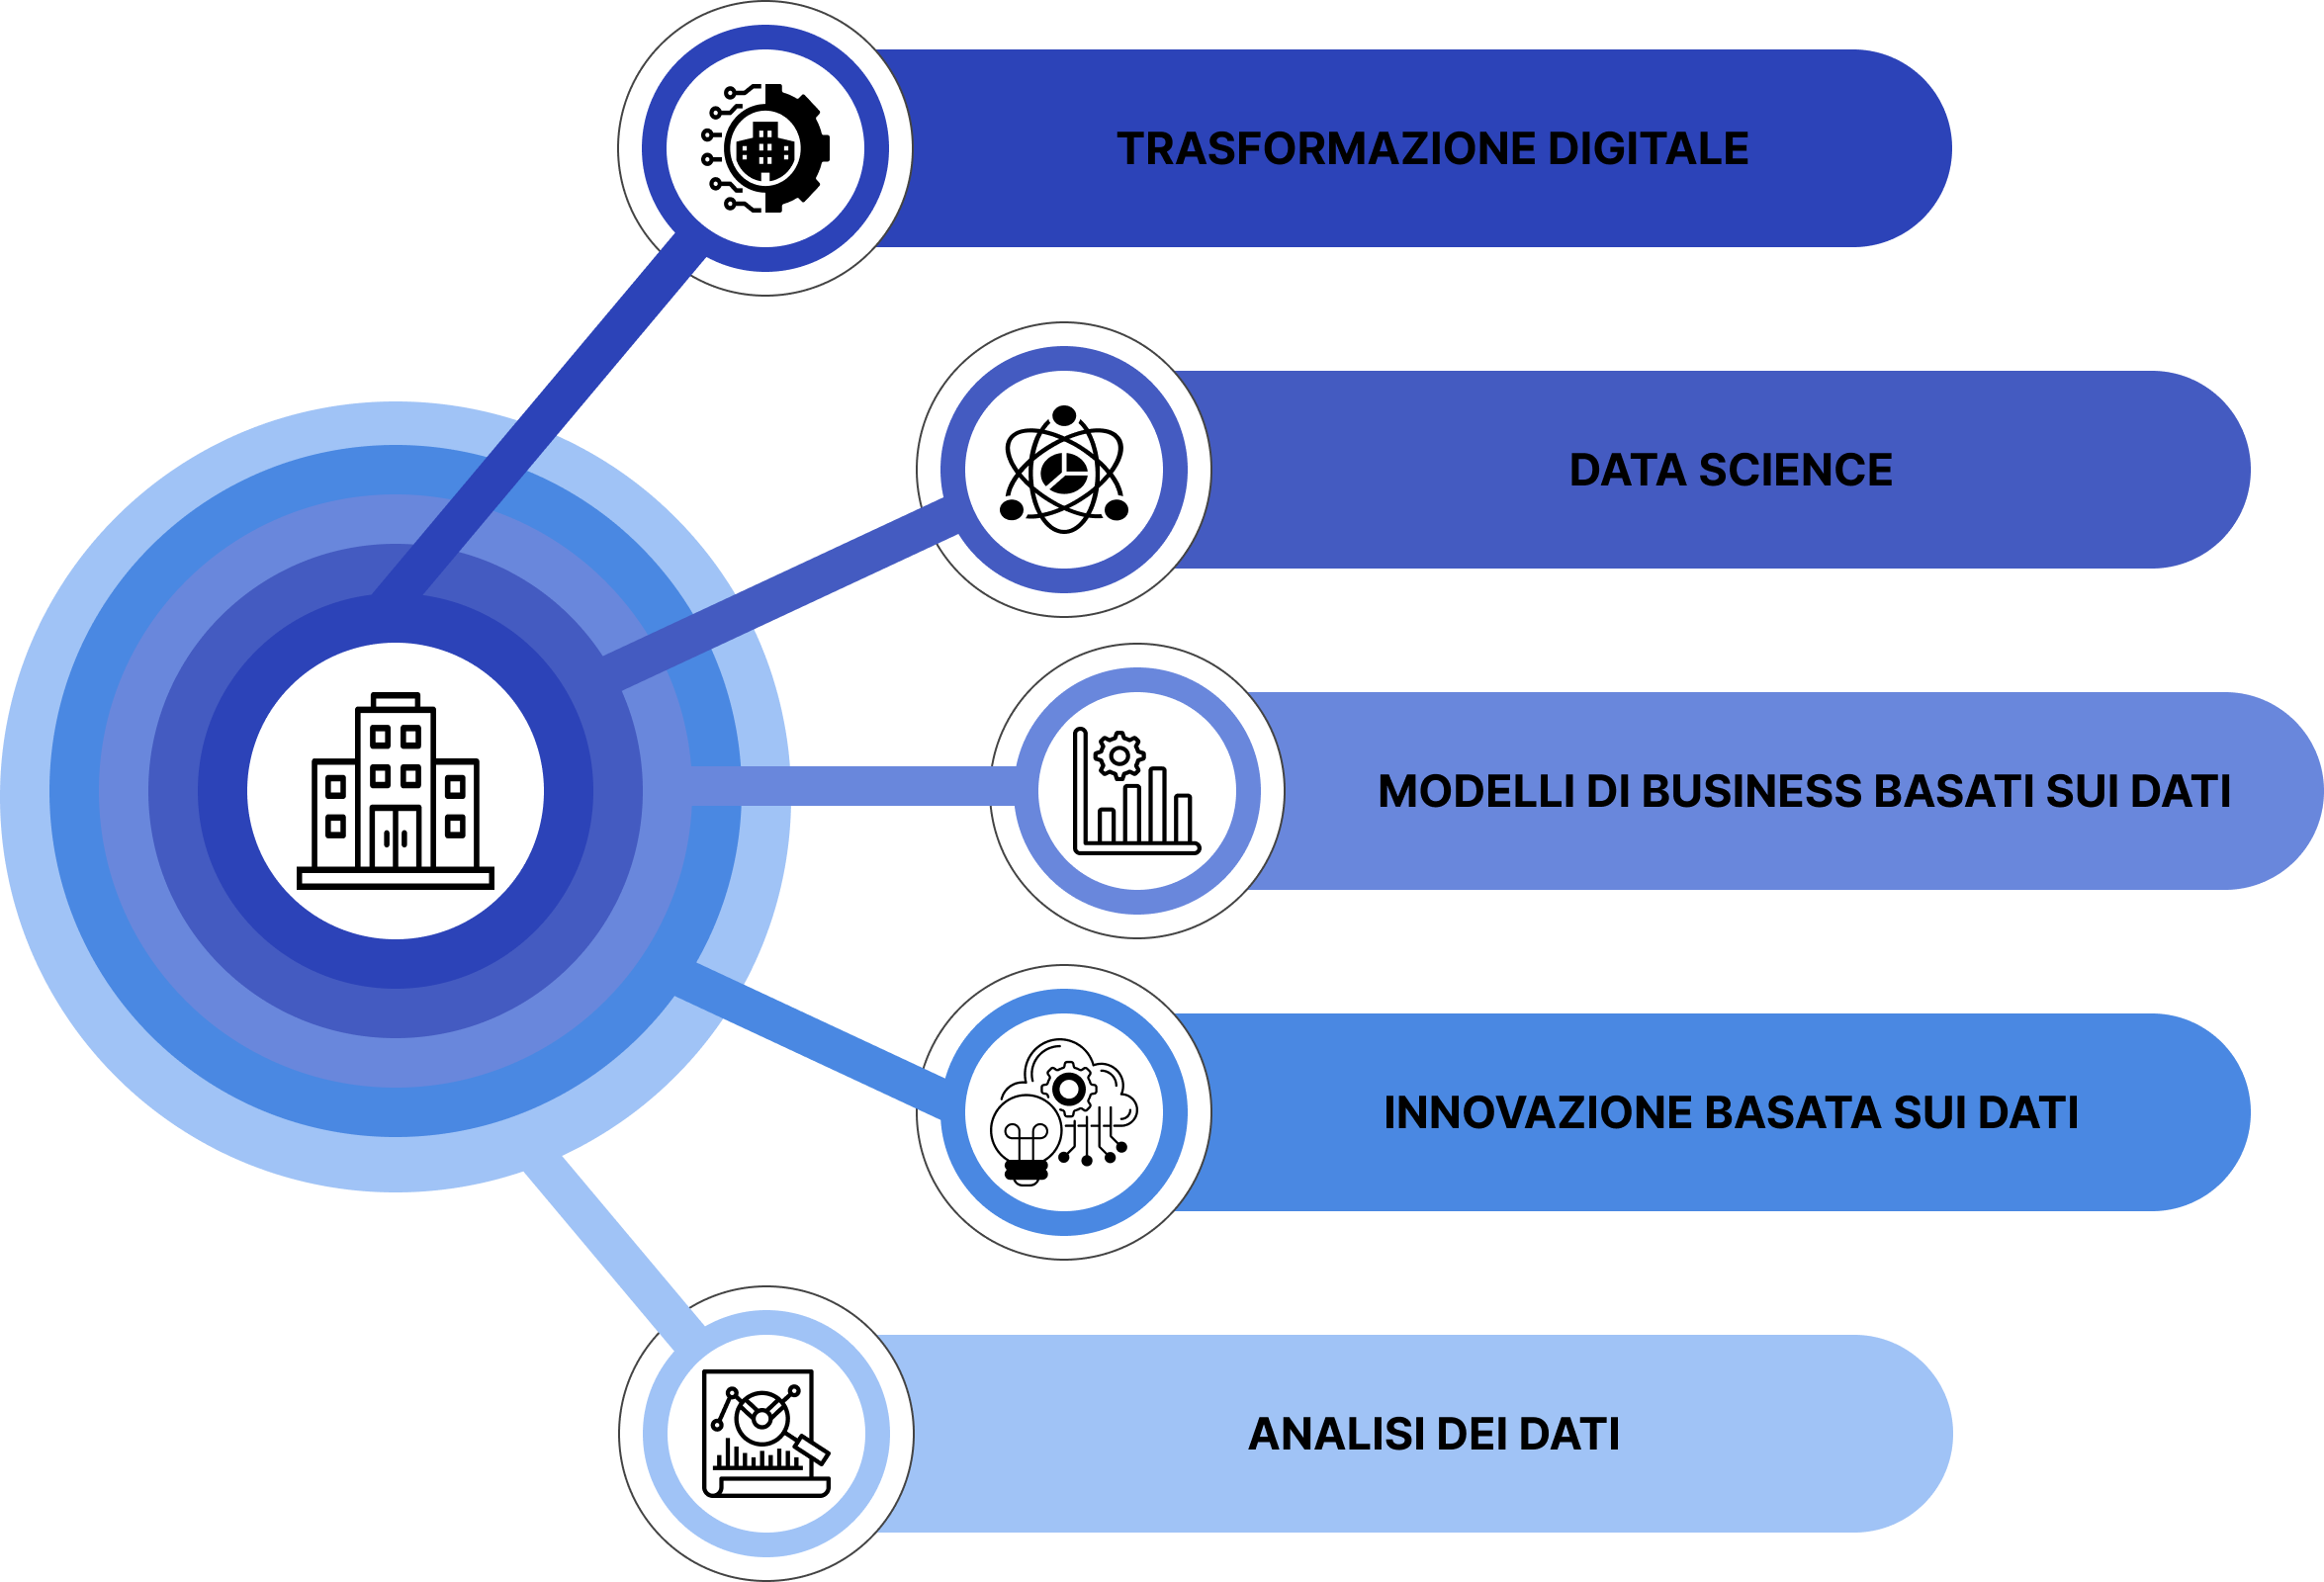
\includegraphics[width=1\linewidth]{figure/capitolo_2/Data-Driven company key points.png}
    \caption{Punti chiave delle aziende Data-Driven oriented}
    \label{fig:Data-Driven company key points}
\end{figure}
\end{comment}

\subsection{Le dimensioni dell'orientamento Data Driven}
Come espresso in precedenza, l'approccio orientato ai dati da parte delle aziende per poter svolgere processi decisionali si basa su diversi punti chiave, tuttavia, non bisogna dare per scontato anche grazie a quali elementi questi vengono svolti. In altre parole, per poter applicare un processo di evoluzione orientato ai dati, un'azienda necessita della stretta collaborazione di tre aree (o fattori) differenti, ovvero:\cite{emerald_data_driven_dimensions}
\begin{itemize}
    \item \textit{Tecnologica}: Corrisponde all'infrastruttura tecnologica necessaria per raccogliere, elaborare e analizzare i dati (includendo hardware, software e sistemi di gestione dei dati).
    \item \textit{Umana}: Corrisponde alle persone coinvolte nel processo di orientazione basato sui dati (includendo le competenze, le abilità e la formazione necessarie per comprendere e utilizzare i dati in modo efficace).
    \item \textit{Manageriale}: Corrisponde alla leadership e la gestione dell'orientamento basato sui dati (includendo strategie, politiche, procedure e processi decisionali che guidano l'uso dei dati all'interno di un'azienda).
\end{itemize}

\begin{comment}
\begin{figure}[!h]
    \centering
    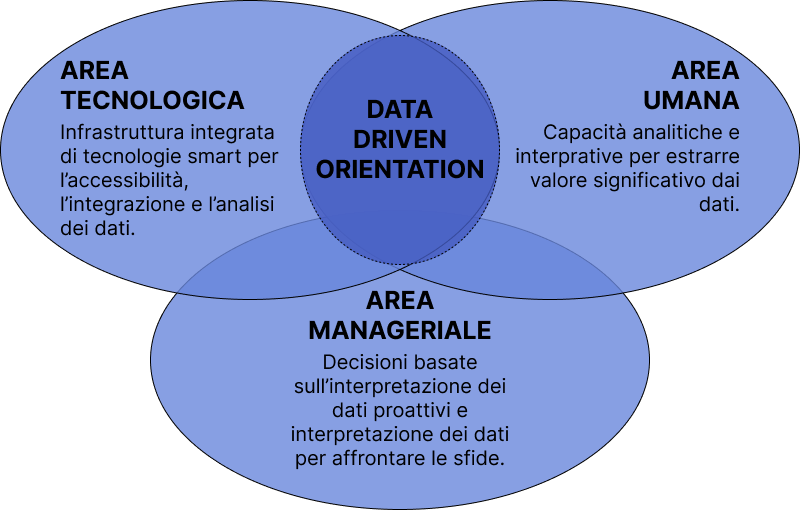
\includegraphics[width=0.75\linewidth]{figure//capitolo_2/Data Driven Orientation Dimensions.png}
    \caption{Dimensioni della Data Driven Orientation}
    \label{fig:Data Driven Orientation Dimensions}
\end{figure}
\end{comment}

\section{Data Governance}
In un mondo come quello odierno in cui i dati sono uno degli asset di maggior valore, poterli gestire in modo efficace ed efficiente diventa fondamentale in qualsiasi ambito e a qualsiasi livello. Proprio per tale motivo l'Unione Europea ha presentato il documento \textit{Data Governance Act}\footnote{Il \textit{Data Governance Act} è una legge che mira a rendere disponibili più dati, regolando il riutilizzo di dati pubblici/protetti, incrementandone la condivisione dei dati attraverso una regolamentazione di nuovi intermediari di dati e incoraggiandone la condivisione a scopi altruistici.}.\cite{europe_data_governance_act}

La \textbf{governance dei dati} (\textit{Data Governance, DG}) promuove la disponibilità, la qualità e la sicurezza di questi all'interno di un'azienda attraverso diverse policy e standard. Questi processi determinano i proprietari, le misure di sicurezza e gli usi previsti per i dati. Nel complesso, l'obiettivo della DG è mantenere dati di alta qualità che siano sicuri e facilmente accessibili per ottenere informazioni aziendali più approfondite.\cite{ibm_data_governance}
Più precisamente, secondo la definizione di Gartner «La governance dei dati è la specificazione dei diritti decisionali e un quadro di responsabilità per garantire il comportamento appropriato nella valutazione, creazione, consumo e controllo dei dati e delle analisi».\cite{gartner_data_governance_definition}

\subsection{Domini della Data Governance}
Come espresso sopra, definire una governance dei dati all'interno di un'azienda permette di indicare chi detiene i diritti decisionali e le responsabilità riguardo gli asset dell'azienda in questione. Pertanto, è importante identificare quali sono i \textit{domini decisionali} di applicazione in modo da assegnare correttamente le responsabilità e i doveri alle persone: principi dei dati, qualità dei dati, metadati, accesso ai dati e ciclo di vita dei dati. I principi dei dati, che sanciscono i confini per l'uso degli asset dei dati che riguardano gli standard aziendali (andando in questo modo a stabilire la direzione per tutti gli altri domini decisionali); la qualità dei dati, che rifinisce la base per come i dati debbano essere interpretati (metadati) e siano accessibili agli utenti (accesso ai dati): infine, la decisione sul ciclo di vita dei dati definisce la loro produzione, conservazione e ritiro, svolgendo un ruolo fondamentale nell'operazionalizzare i principi dei dati nell'ambito delle infrastrutture IT.\cite{data_governance_activities}

\begin{comment}
\begin{figure}[!h]
    \centering
    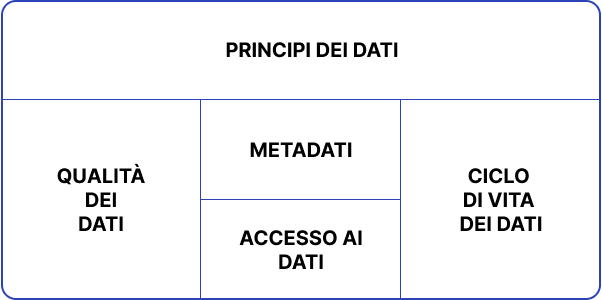
\includegraphics[width=1\linewidth]{figure/capitolo_2/Data Governance Dominions.png}
    \caption{Domini della Data Governance}
    \label{fig:Data Governance Dominions}
\end{figure}
\end{comment}

\subsection{Data Governance Framework}

Un \textit{framework}\footnote{Il termine \textit{framework} è utilizzato per esprimere il concetto di una modalità di struttura, pianificata e permanente, che supporta una prassi, una metodologia, un progetto o un sistema di gestione.\cite{wikipedia_framework_definition}} per la data governance è una raccolta di regole, processi e deleghe di ruolo che garantiscono la privacy e la conformità della gestione dei dati aziendali di una compagnia. D'altronde ogni azienda è guidata da specifici \textit{driver aziendali}, ovvero fattori o processi chiave che sono fondamentali per il successo continuato dell'azienda. Un framework di DG ben pianificato copre ruoli e responsabilità in ambito strategico, tattico e operativo, garantendo che i dati siano affidabili, ben documentati, facili da trovare, conformi, riservati e sicuri.\cite{talend_data_governance_framework}

Per una gestione dei dati su più livelli, è possibile suddividere le attività svolte dalla DG in tre diversi gruppi:\cite{sadas_data_governance_strategy}

\begin{itemize}
    \item \textit{Data Preparation}. Tale attività consiste nell'elaborazione dei dati grezzi provenienti da diverse fonti eterogenee e in una successiva trasformazione degli stessi in possibili dati fruibili dai sistemi aziendali.
    \item \textit{Data Visualization}. Tale attività consiste nell'esplorazione visuale/interattiva e rappresentazione grafica dei dati recuperati, a prescindere dal loro volume e origine.
    \item \textit{Data Cataloguing}. Tale attività consiste nella raccolta dei metadati fisici e di business combinata con strumenti di gestione e ricerca dei dati, fondamentale per svolgere un censimento dei dati a disposizione con le loro relative caratteristiche (annesse connessioni tra dati e concetti di business).
\end{itemize}

\subsection{Vantaggi della governance dei dati}

Di seguito sono riportati i vantaggi che una corretta governance dei dati può comportare all'interno di un'azienda:\cite{google_data_governance}
\begin{itemize}
    \item Prendere decisioni migliori in minor tempo. I dipendenti di un'azienda acquisiscono i dati di cui necessitano per raggiungere e assistere i clienti, progettare e migliorare prodotti e servizi, sfruttando eventuali occasioni.
    \item Migliorare la gestione dei costi. I dati aiutano a gestire le risorse più efficacemente. Grazie ad una corretta gestione sarà inoltre possibile eliminare possibili duplicazioni dei dati, risparmiando spazio e soldi.
    \item Migliorare le conformità normative. Il costante cambiamento del mondo delle leggi e conformità da seguire rende ancora più importante per le organizzazioni una gestione solida e sicura in tale ambito, diminuendone i rischi.
    \item Guadagnare maggiore fiducia da parte dei clienti. La creazione di un sistema preciso, corretto, conforme e ben gestito permette alle aziende di avere un impatto più positivo e rassicurante agli occhi delle persone con cui deve interagire.
    \item Gestire i rischi in modo più semplice. Adoperando una governance corretta è possibile aumentare la sicurezza sull'esposizione dei dati sensibili a sistemi o individui che non dispongono di un'adeguata autorizzazione, sulla violazione della sicurezza da parte di malintenzionati.
    \item Consentire a più persone l'accesso ad una maggiore quantità di dati. Una governance ben strutturata permette ad un numero maggiore di utenti di accedere ai dati per loro necessari in minor tempo, avendo inoltre la certezza della correttezza degli stessi.
\end{itemize}

\subsection{Data Management}

Parlando di governance dei dati, non è possibile non fare riferimento alla macro categoria dell'ambito della gestione dei dati, altrimenti detta nominata come \textbf{Data Management} (\textit{DM}), ovvero la pratica che consente di raccogliere, conservare e utilizzare i dati in modo sicuro, efficiente ed economico. L'obiettivo di tale processo è di aiutare a ottimizzare l'uso dei dati rispetto alle loro relative policy e regolamenti da dover seguire, consentendo in questo modo di prendere decisioni e svolgere azioni che aumentino i vantaggi per un'azienda.\cite{oracle_data_management}

La \textit{DAMA} (\textit{Data Management Association})\footnote{La \textit{Data Management Association} è un'organizzazione internazionale il cui scopo è promuovere concetti e pratiche sulla gestione delle informazioni e dei dati.} definisce le aree di conoscenza, ovvero una categoria di specializzazione che può essere composta da uno o più argomenti, in cui agisce la gestione dei dati. Tali aree sono undici, ovvero:\cite{academiaedu_dama_framework}
\begin{itemize}
    \item \textit{Governance dei dati}: pianificazione, supervisione e controllo sulla gestione dei dati e sull'uso di risorse correlate ai dati;
    \item \textit{Architettura dei dati}: a struttura complessiva dei dati e delle risorse correlate ai dati come parte integrante dell'architettura aziendale;
    \item \textit{Modellazione e Progettazione dei dati}: analisi, progettazione, costruzione, test e manutenzione;
    \item \textit{Memorizzazione e Operazioni sui dati}: dispiegamento e gestione di asset fisici di dati strutturati;
    \item \textit{Sicurezza dei dati}: garantire la privacy, la riservatezza e l'accesso appropriato;
    \item \textit{Integrazione e Interoperabilità dei dati}: acquisizione, estrazione, trasformazione, spostamento, distribuzione, replicazione, federazione, virtualizzazione e supporto operativo;
    \item \textit{Documenti e Contenuti}: archiviazione, protezione, indicizzazione e possibilità di accesso ai dati presenti in fonti non strutturate e rendere tali dati disponibili per l'integrazione e l'interoperabilità con dati strutturati;
    \item \textit{Dati di Riferimento e Dati Principali}: gestire dati condivisi per ridurre la ridondanza e garantirne una migliore qualità attraverso la definizione standardizzata e l'uso di valori dei dati;
    \item \textit{Data Warehousing e Business Intelligence}: gestire l'elaborazione dei dati analitici e consentire l'accesso ai dati di supporto decisionale per la generazione di report e l'analisi;
    \item \textit{Metadati}: raccolta, categorizzazione, gestione, integrazione, controllo, gestione e distribuzione di metadati;
    \item \textit{Qualità dei dati}: definizione, monitoraggio e mantenimento dell'integrità dei dati, oltre che al progressivo miglioramento qualitativo dei dati stessi.
\end{itemize}

%TODO: modificare
\begin{comment}
\begin{figure}[!h]
    \centering
    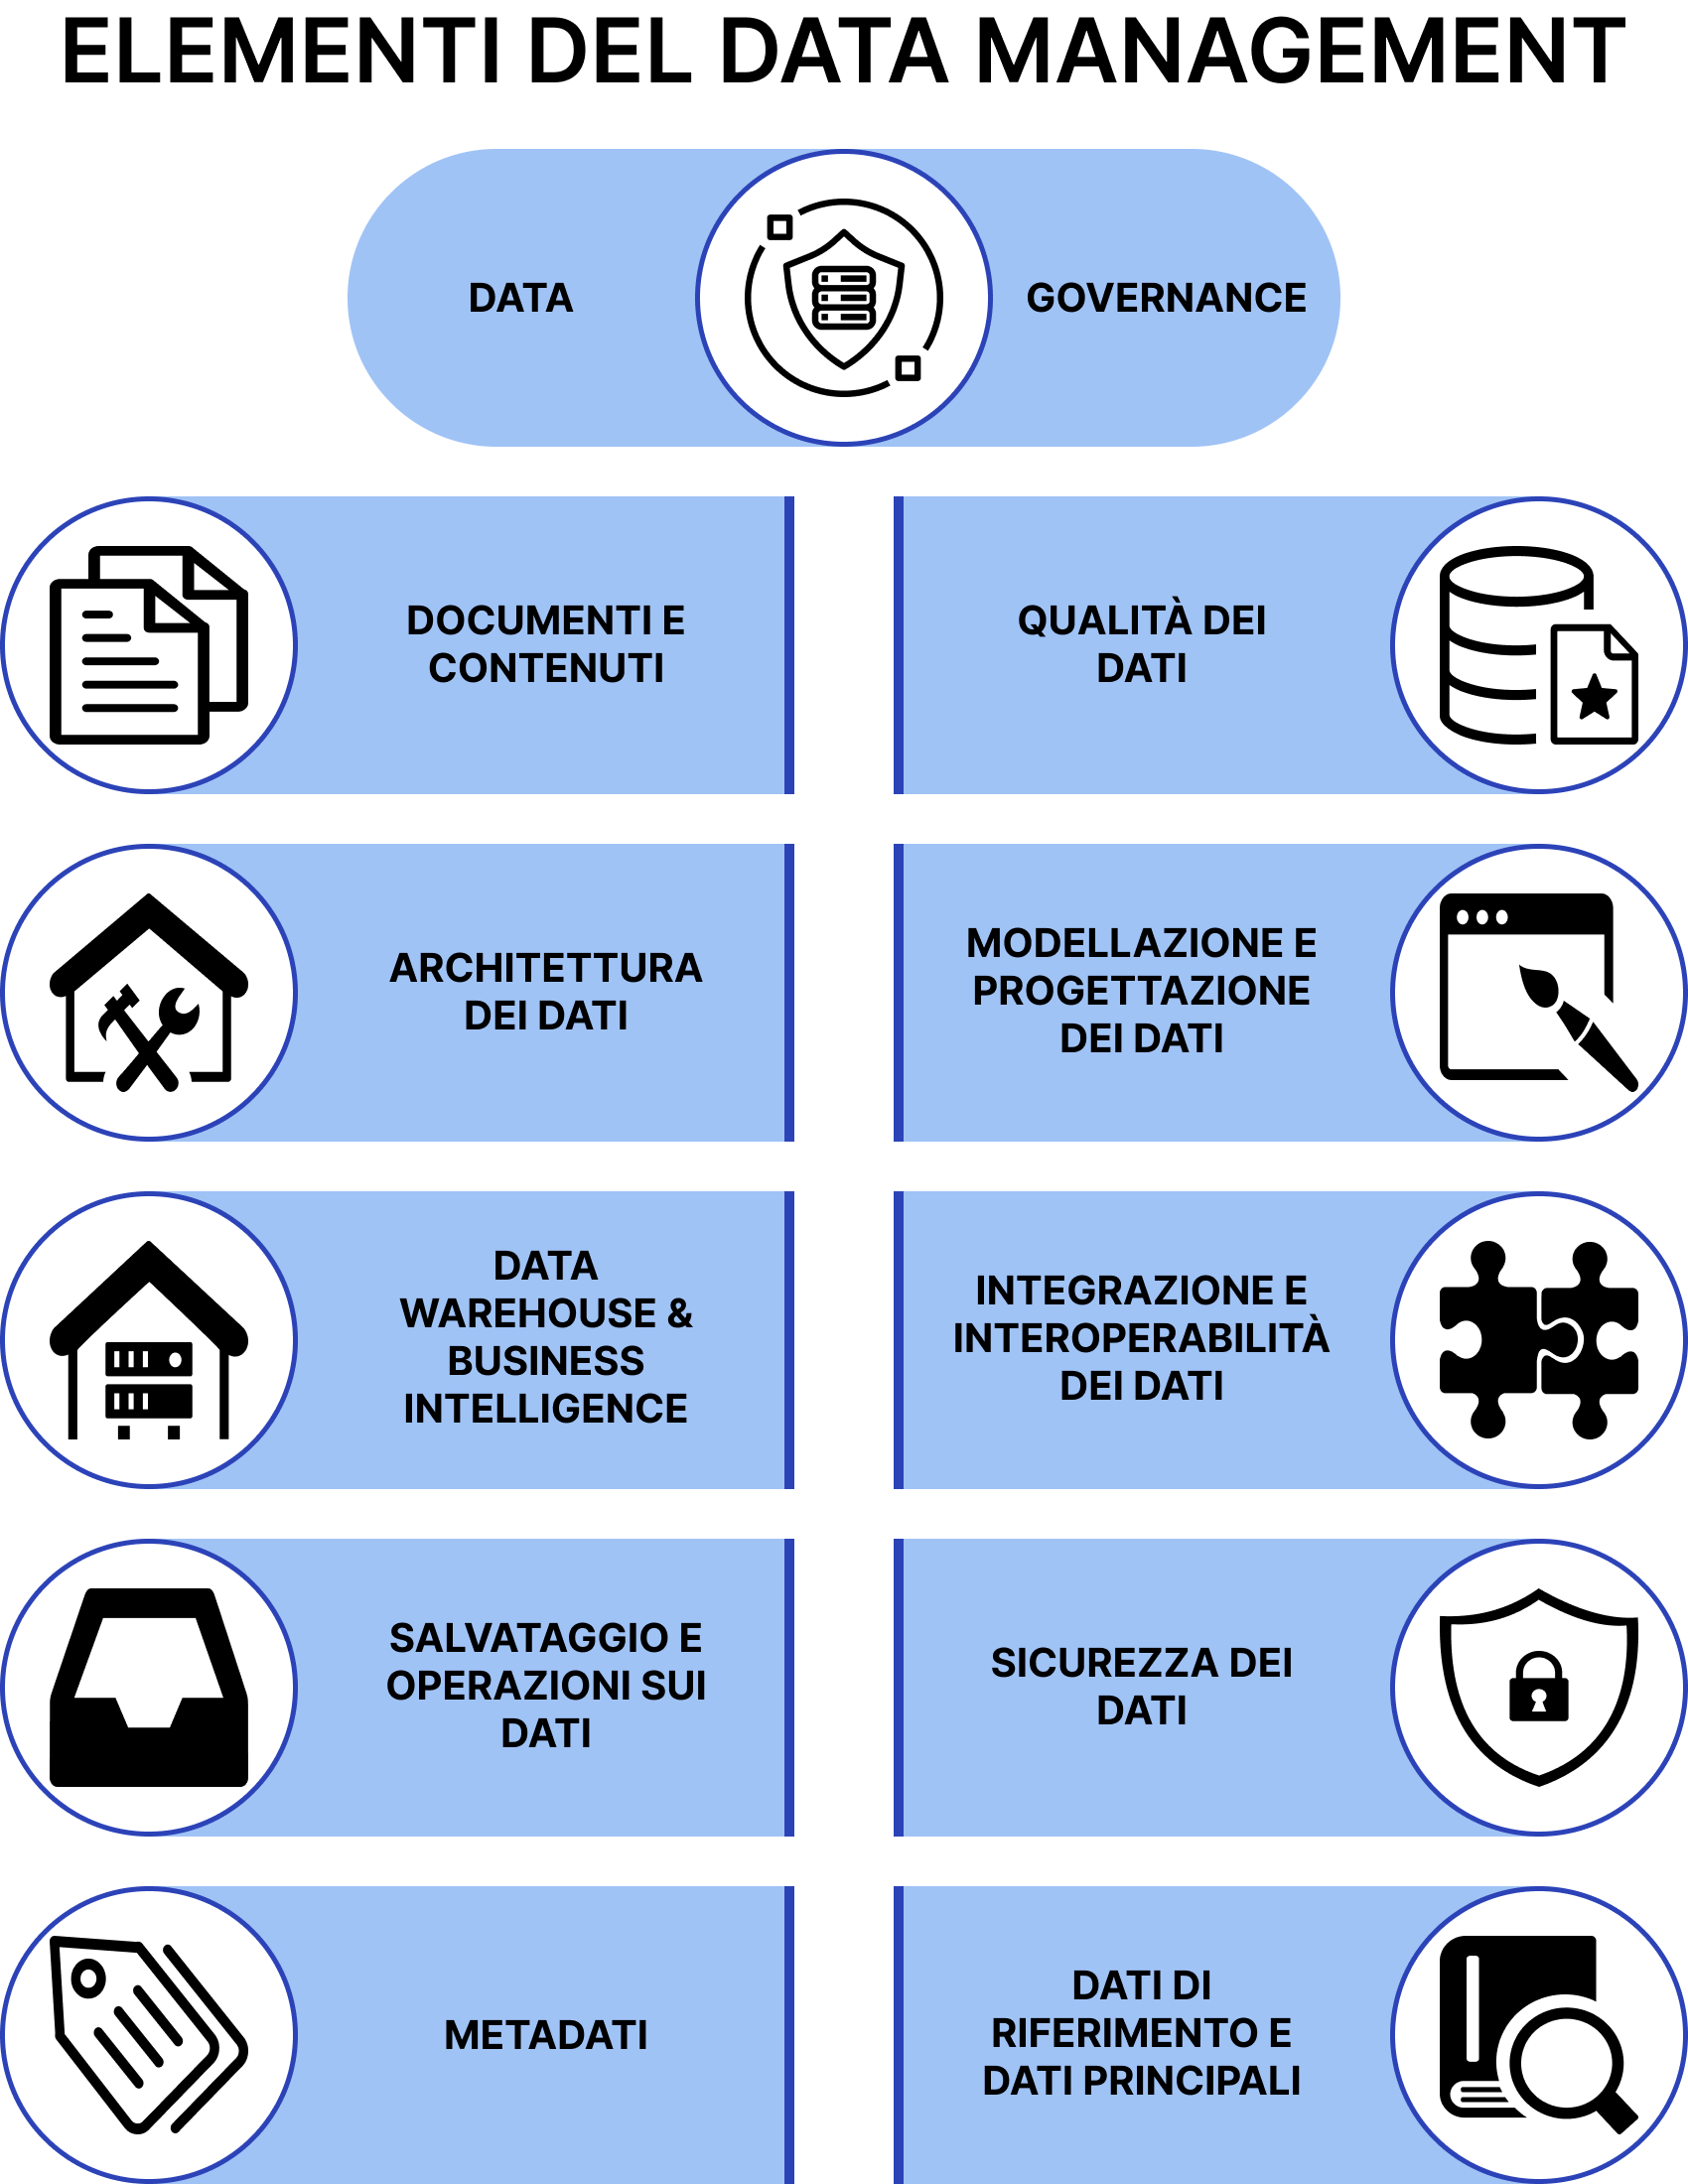
\includegraphics[width=0.75\linewidth]{figure//capitolo_2/Data Management.png}
    \caption{Elementi che compongono il Data Management}
    \label{fig:Data Management}
\end{figure}
\end{comment}
